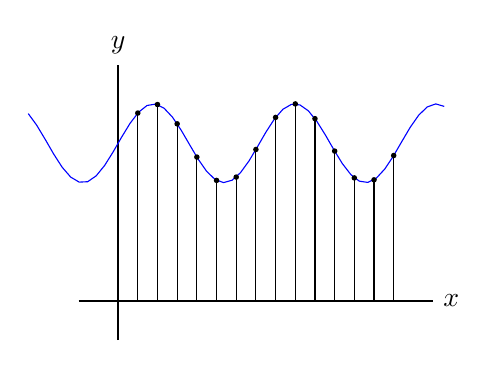
\begin{tikzpicture}
% Axis
\draw[thick] (-0.5,0)--(4,0) node[right]{$x$};
\draw[thick] (0,-.5)--(0,3) node[above]{$y$};

\draw[samples=50, domain=-pi+2:pi+1, blue] plot ({\x},{2+0.5*sin(3.5*\x r)});

\foreach \x in {1, ..., 14}
{
	\draw[samples=10] (	{ \x / 4} , 0) -- ( { \x /4 } , {2+0.5*sin(3.5 * \x / 4  r) } );
	\fill ( {\x / 4} , { 2+0.5*sin(3.5* \x / 4  r) } ) circle [radius=1pt];
}
\end{tikzpicture}
